\section{Własności miary Lebesgue'a w $\Rn$}

Konstrukcja zbioru Vitalego pokazała, gdzie leży nieprzekraczalna granica teorii: nie da się zmierzyć wszystkich podzbiorów $\Rn$ w sposób przeliczalnie addytywny i niezmienniczy na translacje. Wiemy już dokładnie, jak wygląda dziedzina miary Lebesgue'a $\Leb{\Rn}$. Pora zatem zapytać o cechy samej miary: na ile zdefiniowana funkcja $\lambda^n$ jest wyjątkowa? Czy istnieją inne miary spełniające te same postulaty geometryczne? W niniejszym rozdziale wykażemy twierdzenia o jednoznaczności miary Lebesgue'a, zbadamy jej zachowanie przy izometriach i przekształceniach liniowych oraz udowodnimy, że jest ona bezatomowa.

\subsection{Jednoznaczność miary Lebesgue'a}

Podstawowym pytaniem teorii miary jest to, na ile aksjomaty objętości oraz postulaty geometryczne determinują miarę Lebesgue'a. Poniższe twierdzenia pokazują, że miara ta jest wyznaczona jednoznacznie zarówno przez objętość kostek, jak i przez niezmienniczość na translacje wraz z normalizacją na kostce jednostkowej.

\begin{tw}[Jednoznaczność przez objętość kostek]\label{tw:jednoznacznosc_kostki}
    Niech $\mu$ będzie miarą określoną na $\sigma$-algebrze $\Leb{\Rn}$ taką, że dla każdej kostki domkniętej $P \subset \Rn$ zachodzi:
    \begin{equation}
        \mu(P) = V^n(P).
    \end{equation}
    Wówczas $\mu = \lambda^n$ na całej $\sigma$-algebrze $\Leb{\Rn}$.
\end{tw}

\begin{dow}
    Niech $A \in \Leb{\Rn}$ oraz niech $\{P_j\}_{j=1}^\infty$ będzie dowolnym ciągiem kostek domkniętych pokrywającym $A$, tj. $A \subset \bigcup_{j=1}^\infty P_j$. Z przeliczalnej podaddytywności miary $\mu$:
    \begin{equation*}
        \mu(A) \le \mu\left(\bigcup_{j=1}^\infty P_j\right) \le \sum_{j=1}^\infty \mu(P_j) = \sum_{j=1}^\infty V^n(P_j).
    \end{equation*}
    Przechodząc do infimum po wszystkich przeliczalnych pokryciach kostkami domkniętymi, otrzymujemy bezpośrednio:
    \begin{equation*}
        \mu(A) \le \lambda^{*n}(A) = \lambda^n(A).
    \end{equation*}

    Aby dowieść nierówności przeciwnej, załóżmy najpierw, że zbiór $A \in \Leb{\Rn}$ jest ograniczony. Wówczas istnieje duża kostka domknięta $P \supset A$. Zbiór $P \setminus A$ jest mierzalny, więc z pierwszej części dowodu:
    \begin{equation*}
        \mu(P \setminus A) \le \lambda^n(P \setminus A) < +\infty.
    \end{equation*}
    Korzystając ze skończonej addytywności miar na zbiorach o skończonej mierze:
    \begin{equation*}
        \mu(P) - \mu(A) \le \lambda^n(P) - \lambda^n(A).
    \end{equation*}
    Ponieważ z założenia $\mu(P) = V^n(P) = \lambda^n(P) < +\infty$, odejmując tę wartość obustronnie, uzyskujemy:
    \begin{equation*}
        \lambda^n(A) \le \mu(A),
    \end{equation*}
    co daje $\mu(A) = \lambda^n(A)$ dla wszystkich zbiorów ograniczonych.

    Gdy $A$ jest zbiorem nieograniczonym, definiujemy ciąg warstw rozłącznych:
    \begin{equation*}
        A_1 = A \cap [-1, 1]^n, \quad A_j = A \cap \left( [-j, j]^n \setminus [-(j-1), j-1]^n \right) \quad \text{dla } j \ge 2.
    \end{equation*}
    Zbiory $A_j$ są ograniczone, mierzalne i parami rozłączne, a ponadto $A = \bigcup_{j=1}^\infty A_j$. Z przeliczalnej addytywności obu miar:
    \begin{equation*}
        \mu(A) = \sum_{j=1}^\infty \mu(A_j) = \sum_{j=1}^\infty \lambda^n(A_j) = \lambda^n(A),
    \end{equation*}
    co kończy dowód.
\end{dow}


\begin{tw}[Jednoznaczność miary niezmienniczej na translacje]\label{tw:jednoznacznosc_translacje}
    Niech $\mu$ będzie miarą borelowską w $\Rn$ spełniającą dwa warunki:
    \begin{enumerate}
        \item[(i)]
              \textbf{niezmienniczość na translacje}: $\forall A \in \BorelRn, \forall x \in \Rn \colon \quad \mu(x + A) = \mu(A)$;
        \item[(ii)] \textbf{normalizacja na kostce jednostkowej}: $\mu([0, 1)^n) = 1$. \end{enumerate}
    Wówczas $\mu = \lambda^n$ na $\sigma$-algebrze zbiorów borelowskich $\BorelRn$.
\end{tw}
\begin{dow}
    Niech $P_0 = [0, 1)^n$. Dla dowolnej liczby naturalnej $k \wlr 1$ podzielmy każdy z boków kostki $P_0$ na $k$ równych przedziałów postaci $[\frac{i-1}{k}, \frac{i}{k})$.
    Otrzymujemy w ten sposób podział $P_0$ na $k^n$ rozłącznych kostek o krawędzi $\frac{1}{k}$.
    Każda z tych kostek jest translacją kostki $Q_k = [0, \frac{1}{k})^n$.
    Z addytywności i translacyjnej niezmienniczości miary $\mu$:
    \begin{equation*}
        1 = \mu(P_0) = \sum_{j=1}^{k^n} \mu(Q_k) = k^n \mu(Q_k) \implies \mu(Q_k) = \frac{1}{k^n} = \lambda^n(Q_k).
    \end{equation*}
    Dowolną kostkę o krawędziach wymiernych $\prod_{i=1}^n [a_i, b_i)$ (gdzie $a_i = \frac{p_i}{k}, b_i = \frac{q_i}{k}$) można złożyć ze skończonej liczby rozłącznych kostek przystających do $Q_k$. Stąd $\mu(P) = \lambda^n(P)$ dla każdej kostki o wierzchołkach wymiernych. Ponieważ rodzina takich kostek (wraz ze zbiorem pustym) tworzy $\pi$-układ generujący $\sigma$-algebrę borelowską $\BorelRn$, a miary są $\sigma$-skończone (przykryte ciągiem $[-m, m)^n$), z twierdzenia o jednoznaczności rozszerzenia miary na $\pi$-układach (lemat Dynkina o klasie monotonicznej) wynika, że $\mu(B) = \lambda^n(B)$ dla każdego $B \in \BorelRn$.
\end{dow}



\subsection{Własności geometryczne: izometrie i przekształcenia liniowe}

\begin{figure}[htbp]
    \centering
    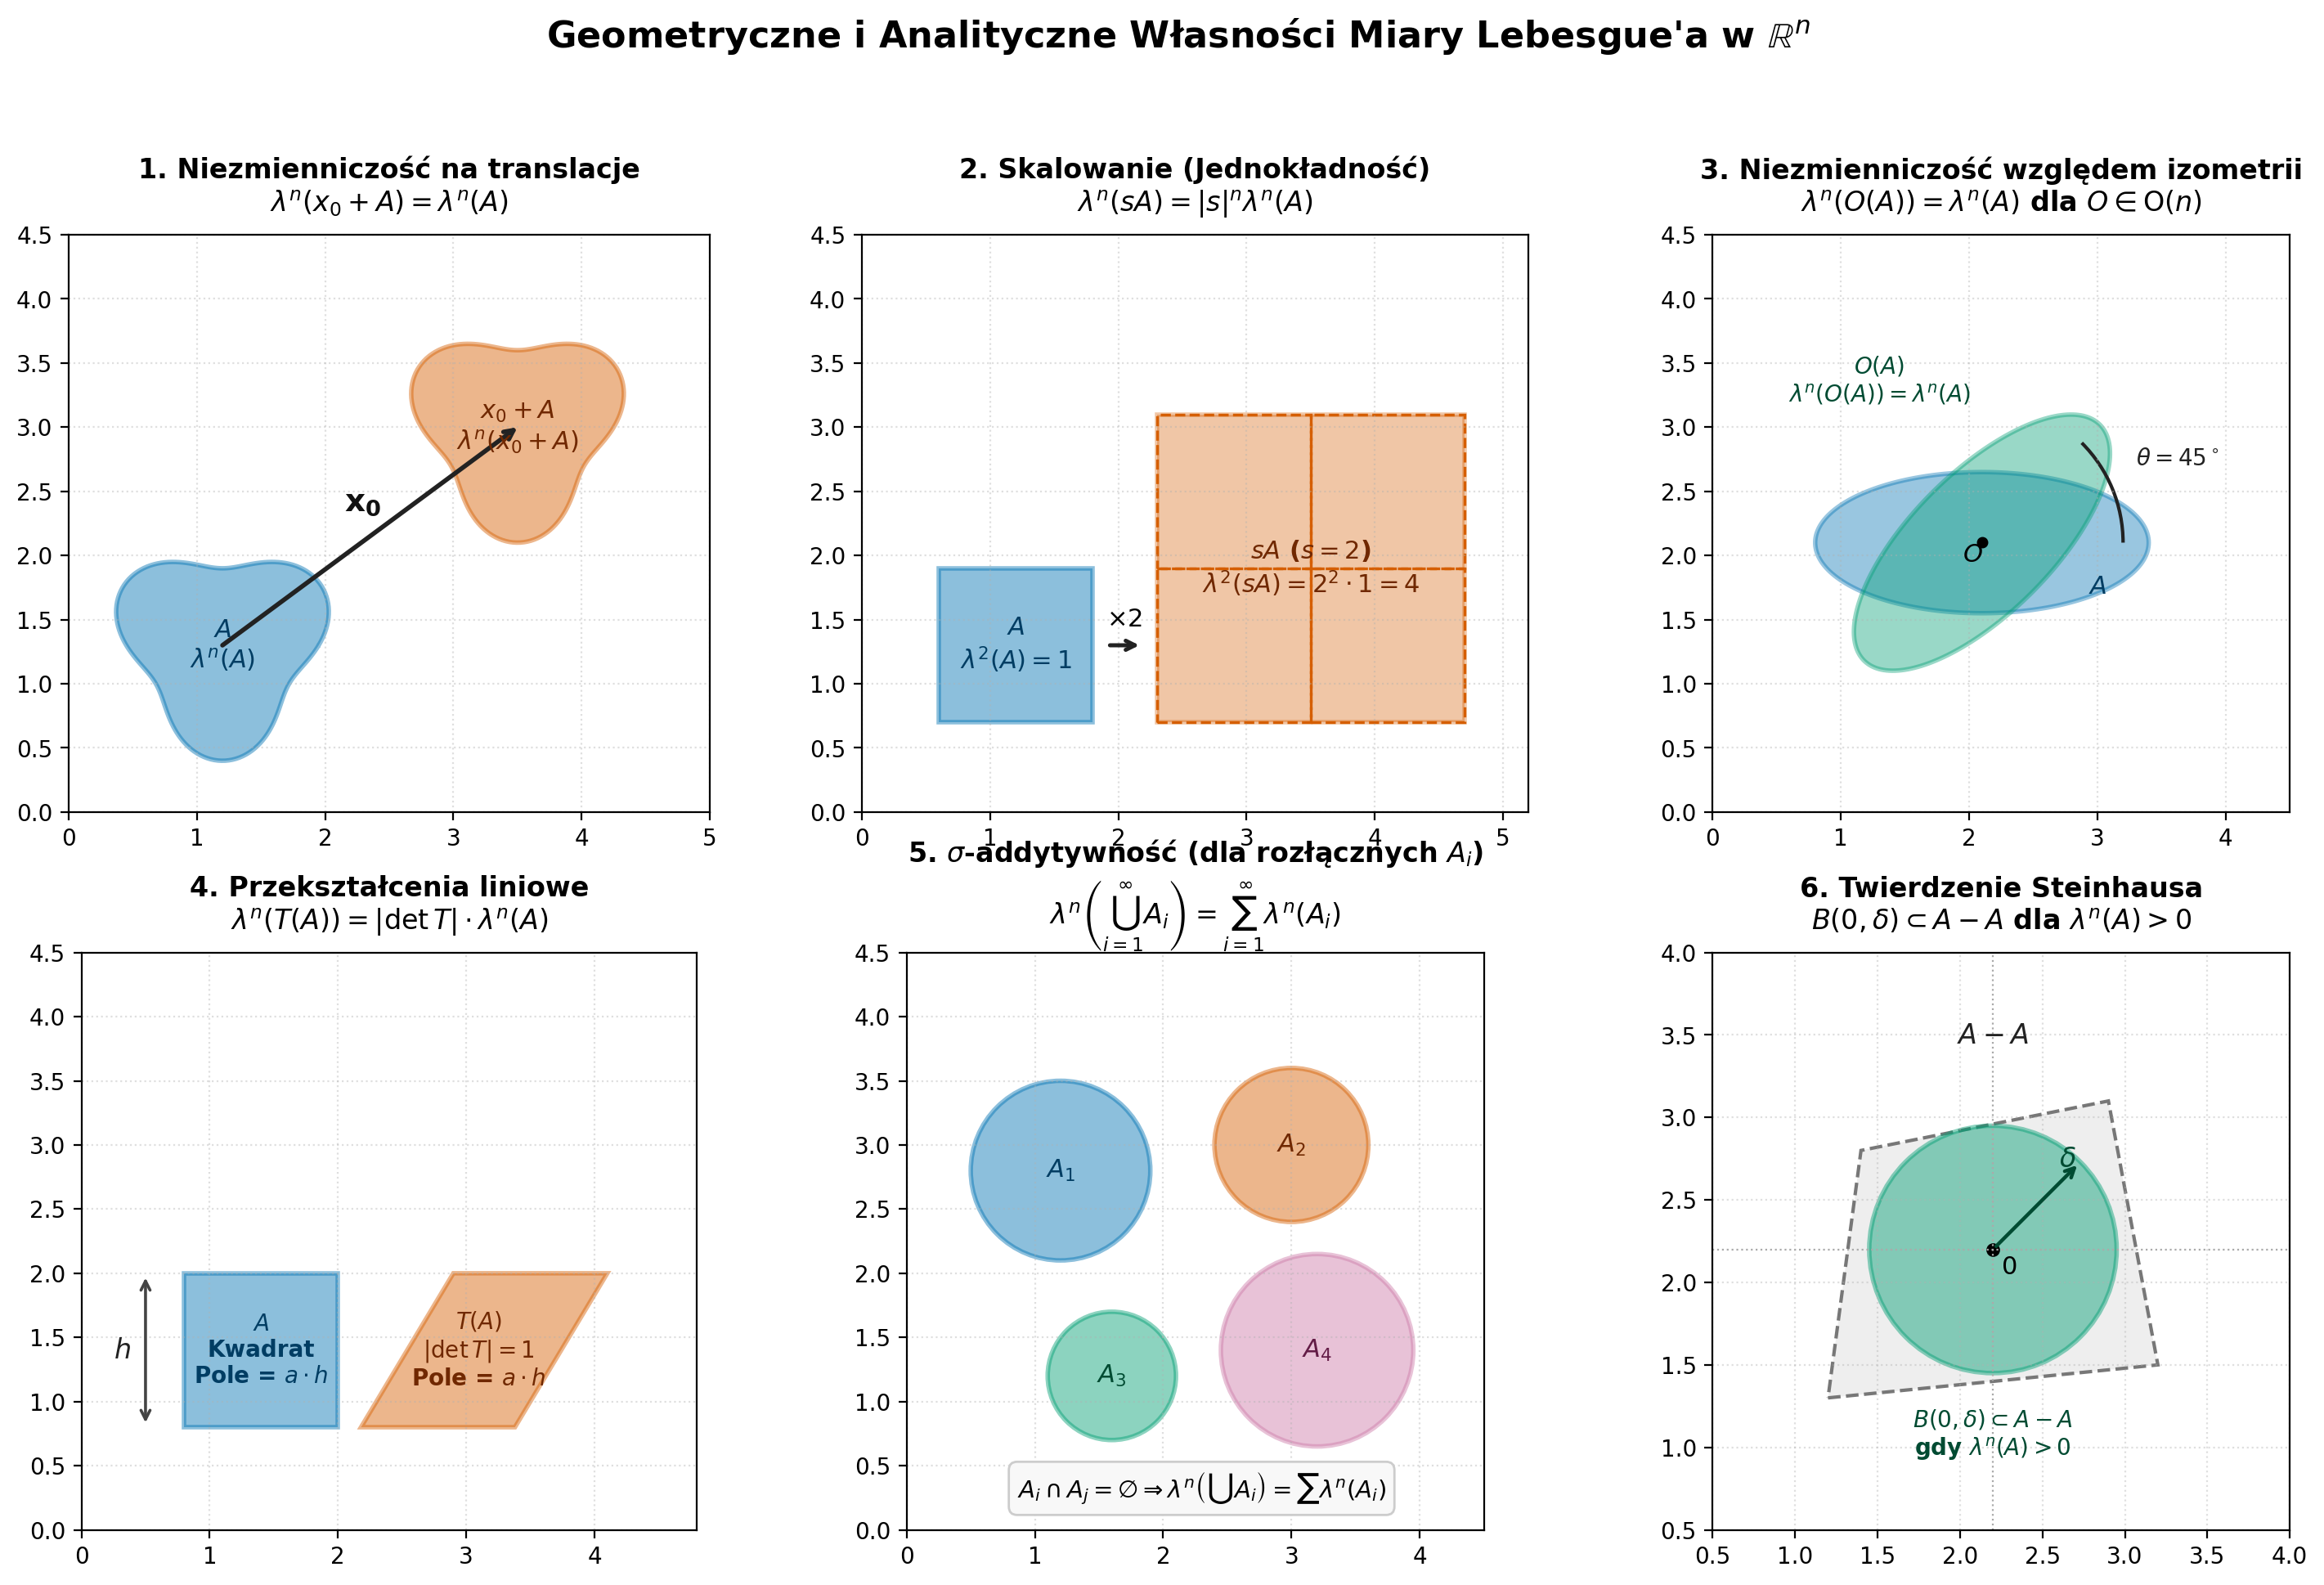
\includegraphics[width=0.95\textwidth]{wlasnosci_miary_lebesguea.png}
    \caption{Geometryczna interpretacja kluczowych własności miary Lebesgue'a w $\Rn$: translacji, skalowania, izometrii, przekształceń liniowych, $\sigma$-addytywności oraz twierdzenia Steinhausa.}
    \label{fig:wlasnosci_miary}
\end{figure}

\begin{tw}[Zachowanie miary przy translacji i skalowaniu]
    Niech $A \in \Leb{\Rn}$, $x_0 \in \Rn$ oraz $s \in \R$. Wówczas:
    \begin{enumerate}
        \item $x_0 + A \in \Leb{\Rn}$ oraz $\lambda^n(x_0 + A) = \lambda^n(A)$;
        \item $sA \in \Leb{\Rn}$ oraz $\lambda^n(sA) = |s|^n \lambda^n(A)$.
    \end{enumerate}
\end{tw}

\begin{tw}[Przekształcenia liniowe]\label{tw:transformacja_liniowa}
    Niech $T \colon \Rn \to \Rn$ będzie operatorem liniowym reprezentowanym przez macierz $M \in M_{n \times n}(\R)$. Jeżeli $A \in \Leb{\Rn}$, to $T(A) \in \Leb{\Rn}$ oraz:
    \begin{equation}
        \lambda^n(T(A)) = |\det T| \cdot \lambda^n(A).
    \end{equation}
\end{tw}

\begin{uwaga}[Intuicja geometryczna dla $n=2$]
    Pełny dowód pomijamy; wyjaśnimy jedynie, skąd bierze się czynnik $|\det T|$ (por.\ Rysunek~\ref{fig:wlasnosci_miary}). Każdą odwracalną macierz $2\times 2$ można zapisać jako złożenie trzech typów prostych przekształceń:
    \begin{enumerate}
        \item[(a)] \textbf{skalowania osi} $(x,y)\mapsto(ax,by)$: kwadrat jednostkowy przechodzi na prostokąt o bokach $|a|$ i $|b|$, więc pole mnoży się przez $|ab| = |\det T|$ (panel~2 rysunku);
        \item[(b)] \textbf{obrotu} (lub symetrii): figura jest przenoszona sztywno, pole się nie zmienia, a $|\det T| = 1$ (panel~3);
        \item[(c)] \textbf{ścinania} $(x,y)\mapsto(x+cy,\,y)$: kwadrat przechodzi na równoległobok o tej samej podstawie i tej samej wysokości, więc pole się nie zmienia, a $\det T = 1$ (panel~4).
    \end{enumerate}
    Ponieważ wyznacznik złożenia jest iloczynem wyznaczników, a pola mnożą się w ten sam sposób, dla każdego prostokąta $P$ otrzymujemy $\lambda^2(T(P)) = |\det T|\,\lambda^2(P)$; przybliżając dowolny zbiór mierzalny pokryciami prostokątami, dostajemy tę równość dla wszystkich $A \in \Leb{\R^2}$. Gdy $\det T = 0$, obraz $T(\R^2)$ jest prostą lub punktem, a więc zbiorem miary zero.
\end{uwaga}

\begin{wn}[Niezmienniczość względem izometrii]
    Każda izometria przestrzeni euklidesowej $\Phi \colon \Rn \to \Rn$ ma postać $\Phi(x) = Ox + x_0$, gdzie $O \in \mathrm{O}(n)$ jest macierzą ortogonalną ($O^T O = I$), a $x_0 \in \Rn$. Ponieważ $\det O = \pm 1$, dla każdego zbioru $A \in \Leb{\Rn}$ zachodzi:
    \begin{equation}
        \lambda^n(\Phi(A)) = |\det O| \cdot \lambda^n(A) = \lambda^n(A).
    \end{equation}
    W szczególności miara Lebesgue'a jest niezmiennicza na obroty wokół środka układu współrzędnych oraz symetrie zwierciadlane.
\end{wn}

\subsection{Własności strukturalne: bezatomowość i własność Darboux}

\begin{defi}[Atom miary]
    Niech $(X, \mathcal{M}, \mu)$ będzie przestrzenią z miarą. Zbiór $A \in \mathcal{M}$ o mierze $\mu(A) > 0$ nazywamy \textbf{atomem miary} $\mu$, jeżeli dla każdego podzbioru mierzalnego $B \in \mathcal{M}, B \subset A$ zachodzi:
    \begin{equation}
        \mu(B) = 0 \quad \text{albo} \quad \mu(B) = \mu(A).
    \end{equation}
    Miarę $\mu$ nazywamy \textbf{bezatomową}, jeżeli nie posiada ona żadnych atomów.
\end{defi}

\begin{tw}[Bezatomowość miary Lebesgue'a]
    Miara Lebesgue'a $\lambda^n$ w $\Rn$ jest miarą bezatomową.
\end{tw}

\begin{dow}
    Niech $A \in \Leb{\Rn}$ spełnia $\lambda^n(A) > 0$. Ponieważ $A = \bigcup_{m=1}^\infty \left(A \cap [-m, m]^n\right)$, z ciągłości miary z dołu istnieje $m \in \N$ takie, że zbiór $A_m := A \cap [-m, m]^n$ ma miarę $0 < \lambda^n(A_m) \mlr (2m)^n < +\infty$. Rozważmy półprzestrzenie $H_t = \{x \in \Rn \colon x_1 \mlr t\}$ dla $t \in \R$ i zdefiniujmy funkcję:
    \begin{equation*}
        f(t) := \lambda^n(A_m \cap H_t).
    \end{equation*}
    Funkcja $f$ jest niemalejąca, $f(t) = 0$ dla $t < -m$ oraz $f(t) = \lambda^n(A_m)$ dla $t \wlr m$. Ponadto $f$ jest ciągła, gdyż dla dowolnych $t_1 < t_2$:
    \begin{align*}
        0 \mlr f(t_2) - f(t_1) & = \lambda^n(A_m \cap \{x \colon t_1 < x_1 \mlr t_2\})                     \\
                               & \mlr \lambda^n\left([t_1, t_2] \times [-m, m]^{n-1}\right) = (2m)^{n-1}(t_2 - t_1).
    \end{align*}
    Z własności Darboux dla funkcji ciągłej $f$ istnieje punkt $t_0 \in \R$ taki, że:
    \begin{equation*}
        f(t_0) = \lambda^n(A_m \cap H_{t_0}) = \frac{1}{2} \lambda^n(A_m).
    \end{equation*}
    Kładąc $B = A_m \cap H_{t_0} \subset A$, otrzymujemy podzbiór mierzalny o mierze $0 < \lambda^n(B) = \frac{1}{2}\lambda^n(A_m) < \lambda^n(A_m) \mlr \lambda^n(A)$. Zbiór $A$ nie jest więc atomem, co dowodzi bezatomowości miary $\lambda^n$.
\end{dow}

\begin{wn}[Własność Darboux dla miary Lebesgue'a]
    Dla każdego zbioru mierzalnego $A \in \Leb{\Rn}$ oraz dowolnej liczby rzeczywistej $c$ spełniającej $0 \le c \le \lambda^n(A)$ istnieje zbiór mierzalny $B \subset A$ taki, że:
    \begin{equation}
        \lambda^n(B) = c.
    \end{equation}
\end{wn}

\begin{uwaga}[Twierdzenie Steinhausa]
    Dla zbioru $A \subset \Rn$ jego \textbf{zbiorem różnic} nazywamy zbiór $A - A := \{x - y \colon x, y \in A\}$. H.~Steinhaus udowodnił w 1920 roku, że jeżeli $A \in \Leb{\Rn}$ oraz $\lambda^n(A) > 0$, to zbiór $A - A$ zawiera pewną kulę otwartą $B(0, \delta)$, $\delta > 0$. Z twierdzenia tego wynika alternatywny dowód niemierzalności zbioru Vitalego $V$ z Twierdzenia~\ref{tw:vitali}: gdyby $V$ był mierzalny, miałby dodatnią miarę, tymczasem $(V - V) \cap \Q = \{0\}$, więc $V - V$ nie zawiera żadnego przedziału.
\end{uwaga}
